\documentclass[a4paper]{scrartcl}

\usepackage[ngerman]{babel}
\usepackage[utf8]{inputenc}
\usepackage[T1]{fontenc}
\usepackage{graphicx}
\usepackage{tabularx}

\title{Compi-Flick: Use-Cases}
\author{Damien Flury}
\date{9. September 2020}

\begin{document}
\maketitle
\begin{figure}
  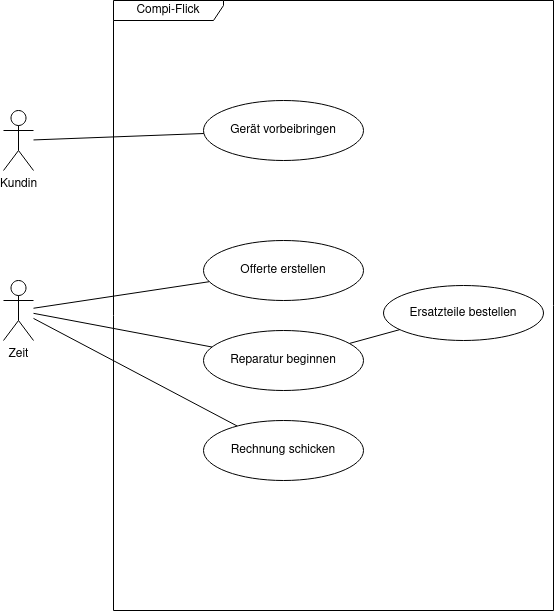
\includegraphics[width=\textwidth]{images/compi-flick-use-case.png}
  \caption{Use-Case-Diagramm}
\end{figure}

\section{Use Cases}
\subsection{Gerät vorbeibringen}
\begin{tabularx}{\textwidth}{|l|X|}
  \hline
  Motivation & Dieser Anwendungsfall wird von
  der Kundin ausgelöst. Er ist wichtig, dass eine
  Reparatur starten kann. \\ \hline
  Auslöserin & Die Kundin \\ \hline
  Input & Das Gerät und eventuelle Informationen, welche
  die Kundin hat (z.B. Schadenursache) sind Argumente, welche
  die Kundin ans System übergibt. \\ \hline
  Rate & Einmal pro Reparatur \\ \hline
  Output & 
\end{tabularx}

\end{document}